\documentclass{article}
\usepackage[portrait, margin=1in]{geometry}
\usepackage{graphicx} 
\graphicspath{{/Users/danpost/consumer_sentiment/output/umich_figures/macro_vars}}
\usepackage{amsmath}
\usepackage{hyperref}
\usepackage{threeparttable}

\title{University of Michigan's Surveys of Consumers Respondents' Sensitivity to Macroeconomic Conditions}
\author{Daniel Posthumus}

\begin{document}
\maketitle

\section{Summary}
 

\section{Methodology}
\subsection{Sources/Links}
\begin{itemize} 
	\item \href{https://data.sca.isr.umich.edu/fetchdoc.php?docid=75440}{List of questions in survey}
	\item \href{https://data.sca.isr.umich.edu/fetchdoc.php?docid=75439}{Time series codebook of variables with descriptions}
	\item \href{https://data.sca.isr.umich.edu/technical-docs.php}{Survey Technical Documentation}
\end{itemize} 
\subsection{Catalog of Variables}
For each regressor, I compute two models:
\begin{enumerate} 
	\item Using monthly \% difference for the regressor
	\item Using year-over-year \% difference for the regressor
\end{enumerate}
\begin{table}[h!]
\begin{threeparttable}
\begin{tabular}{|l|l|l|l|}
\hline
\textbf{Section} 							& \textbf{Question on Survey} 	& \textbf{Outcome Variable} 	& \textbf{Regressor} 		\\ \hline
Government Economic Policy      			& GOVT      				& GOVT\_R 				&   NA  				\\ \hline
Personal Financial Conditions      			& PAGO      				& PAGO\_R  				&   NA 				\\ \hline
Broad Business Conditions     				& BAGO      				& BAGO\_R 				&   NA 				\\ \hline
Home-Buying Conditions		     			& HOM      				& HOM\_R  				&   Zillow Home Index\tnote{1}	\\ \hline
Unfavorable News Coverage of Inflation    	& NEWS      				& NEWSRN\_U\_PRI  		&   All-Urban CPI\tnote{2}		\\ \hline
Likelihood of Positive Stock Market Return 	& PSTK     				& PSTK\_MEAN  			&   S\&P 500\tnote{3}	 \\ \hline
Real Household Income     				& RINC      				& RINC\_R 				&   Real Family Income\tnote{4} \\ \hline
Car-Buying Conditions      					& CAR      				& VEH\_R 				&   Used Car CPI\tnote{5} \\ \hline
\end{tabular}
\begin{tablenotes} 
\footnotesize
\item[1] Source: \href{https://fred.stlouisfed.org/series/USAUCSFRCONDOSMSAMID}{FRED} 
\item[2] Source: \href{https://fred.stlouisfed.org/series/CPIAUCSL}{FRED}
\item[3] Source: \href{https://finance.yahoo.com/quote/\%5EGSPC/}{Yahoo Finance} -- note: I used the closing value for this series at the end of each month.
\item[4] Source: \href{https://fred.stlouisfed.org/series/A229RX0}{FRED}
\item[5] Source: \href{https://fred.stlouisfed.org/series/CUSR0000SETA02}{FRED} 
\end{tablenotes}
\end{threeparttable}
\end{table}

\subsection{Calculation of Outcome Variables, by Partisan Affiliation}
On the Consumer Survey, questions about attitudes towards economic factors, say var $x$, typically ask respondents to select one of the following: (1) Positive, (3) Same/Neutral, or (5) Negative. Then the corresponding time series variable $x$\_R is calculated by subtracting the shares of respondents that answered in the negative to $x$ from the share that answered in the positive to $x$, and adding 100. In the aggregated time series, this figure is \textit{not} reported by partisan affiliation; however, I recreated this number and plotted the time-series by partisan affiliation below. In chart titles, I refer to the variable $x$\_R as the `net' attitude corresponding to each macroeconomic condition. These are thus grouped by month-year and partisan affiliation.\footnote{Note that lines in bold are 6-month moving averages of the net attitude and the fainter lines are the non-adjusted figures. \\ This was my approach for the variables corresponding to voters' attitudes towards the economy. However, for predicted likelihood of a positive investment in the stock market, I simply found the mean by month-year and partisan affiliation. Then for respondents' reported unfavorable news coverage of inflation, I calculated the share of respondents who responded that selected unfavorable news coverage of inflation to at least one of the two questions asking respondents what news coverage of business conditions they had heard.}

\subsection{Modeling Respondents' Sensitivity -- Aggregate Approach}
We want to go beyond just comparing attitudes over time, and instead want to understand what role real-world, observed macroeconomic changes play in respondents' expectations or attitudes. For the aggregate approach, I take the time-series aggregates described above and I ran separate regressions by (1) partisan affiliation,  (2) whether Biden was president or president-elect, and (3) using monthly vs. year-over-year \% percent changes in the regressor, estimating the following equation:\footnote{I'm using Biden's election as the beginning of his `presidency', so that the dummy variable biden = 1 for all dates starting with December 2020.}
\begin{gather} 
	\text{OUTCOME}_{p,t,m} = \alpha_0 + \beta_1 \text{REGRESSOR}_{t,h} *\text{BIDEN}_t + \epsilon_{p,t,h,m}
\end{gather} 
where $p \in \{\text{democrats}, \text{republicans}\}$, $t$ is month-year, $m \in \{\text{aggregate model}, \text{micro model}\}$, \\
and $h \in \{\text{monthly \% change}, \text{year-over-year \% change}\}$.

\subsection{Modeling Respondents' Sensitivity -- Micro Approach}
The advantage of using the aggregate approach is that our outcome variable is more precise, capturing \textit{net} attitudes. The disadvantage is that the sample size is small.\footnote{For Biden-era regressions, the sample size is 42 and for non-Biden-era regressions, the sample size is 39.} Instead, we can use individual-level attitudes and beliefs in a micro model.\footnote{In the Micro model, the Biden-era sample sizes for Democrats, Republicans, and Independents are 7,305; 6,750; and 10,112; respectively. For non-Biden-era samples, the sizes are 6,776; 6,319; and 8,722; respectively.} For this model, I use dummy outcome variables capturing whether a respondent responded positive to a question about attitudes, or a dummy for whether they responded to hearing unfavorable news coverage of inflation. Only for the predicted likelihood of a positive investment in the stock market, I left the respondent's answer unchanged. I ran separate regressions by 1) partisan affiliation,  2) whether Biden was president or president-elect, 3) using monthly vs. year-over-year \% percent changes in the regressor, estimating the following equation: 
\begin{gather} 
	\text{OUTCOME}_{p,t,i,m} = \alpha_0 + \beta_1 \text{REGRESSOR}_{t,h} *\text{BIDEN}_t + \epsilon_{p,t,h,i,m}
\end{gather} 
where $i$ is the individual survey respondent. 

\section{Attitudes Towards Government Economic Policy}
\centering 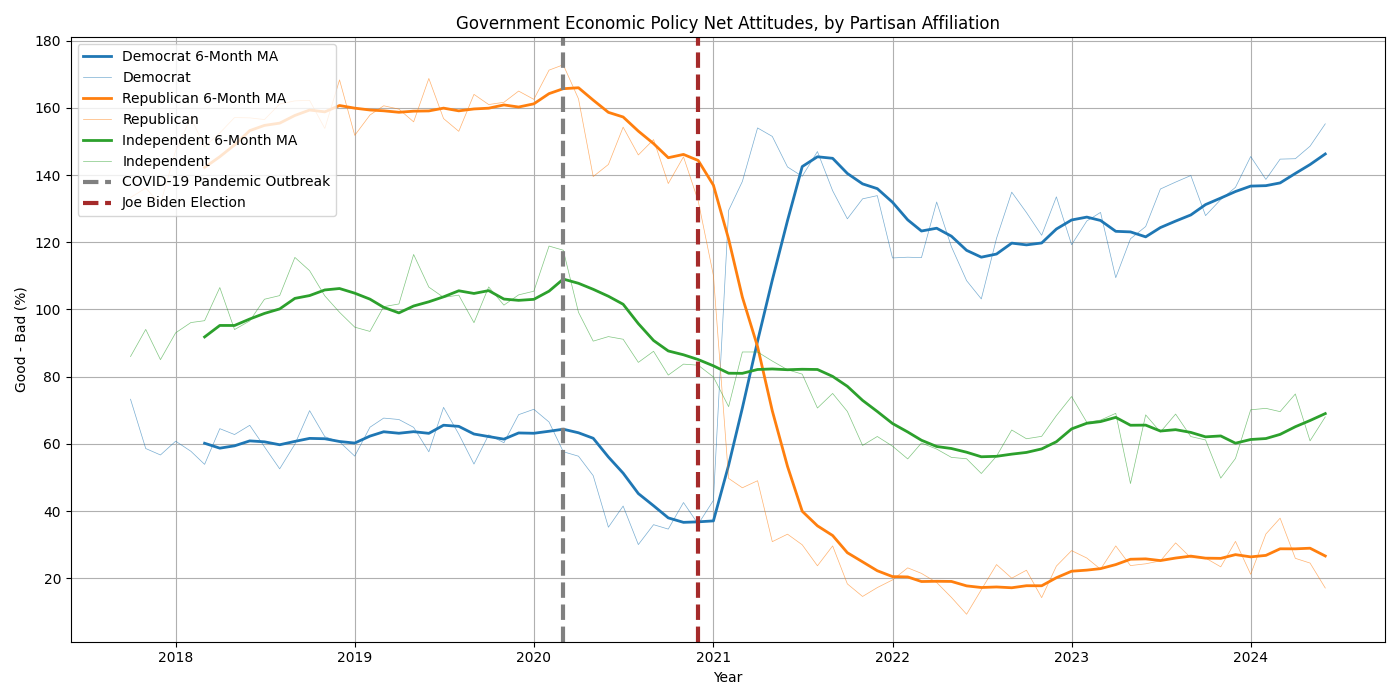
\includegraphics[width=5.5in]{govt_r_time_series.png}\\
\raggedright Democrats' and Republicans' attitudes towards government economic policy nearly exactly inverted upon Joe Biden's election. Since the onset of COVID-19, Independents' attitudes towards government economic policy have steadily until bottoming out in mid-2022.

\section{Attitudes Towards Personal Financial Conditions}
\centering 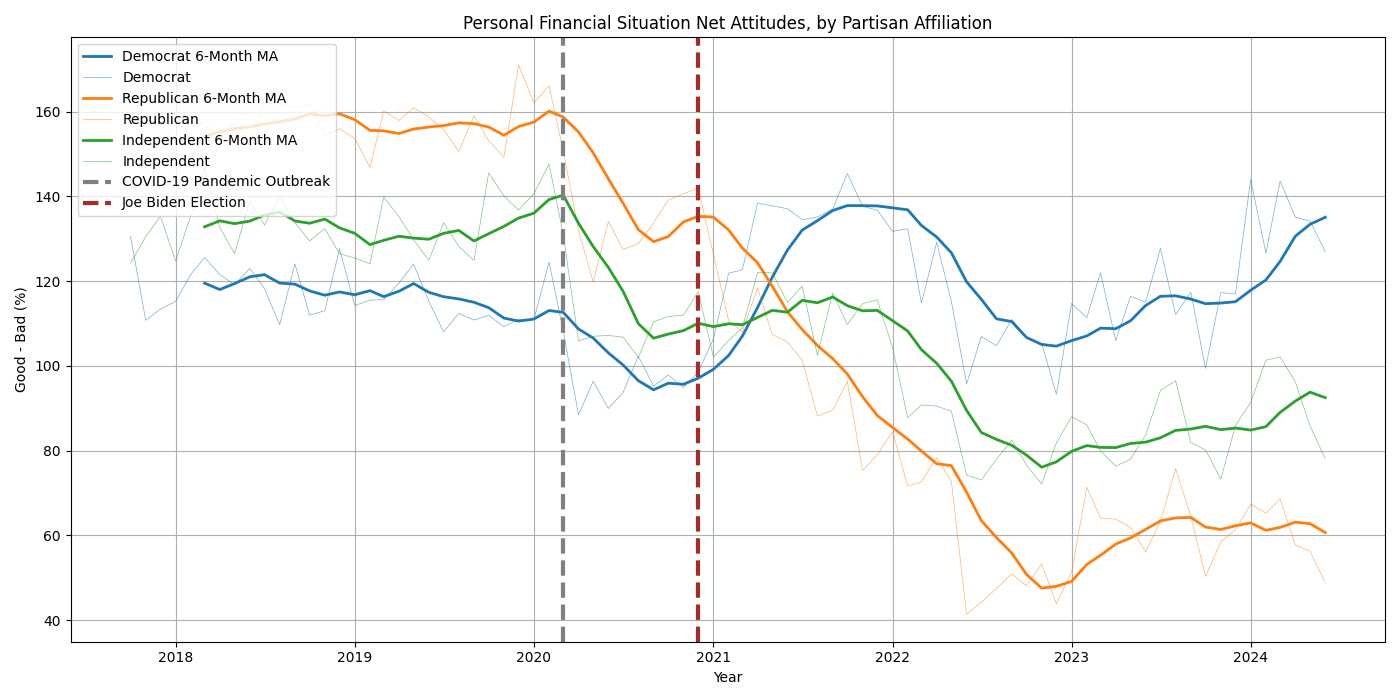
\includegraphics[width=5.5in]{pago_r_time_series.png}\\
\raggedright There were large decreases in PAGO\_R coinciding with the onset of COVID. Then Democrats' conditions improved following Biden's election, while Republicans' fell and Independents' stagnated. With the onset of inflation in 2022, conditions worsened across parties, with some rebound occurring in late 2022 for all parties.

\section{Attitudes Towards Broad Business Conditions}
\centering 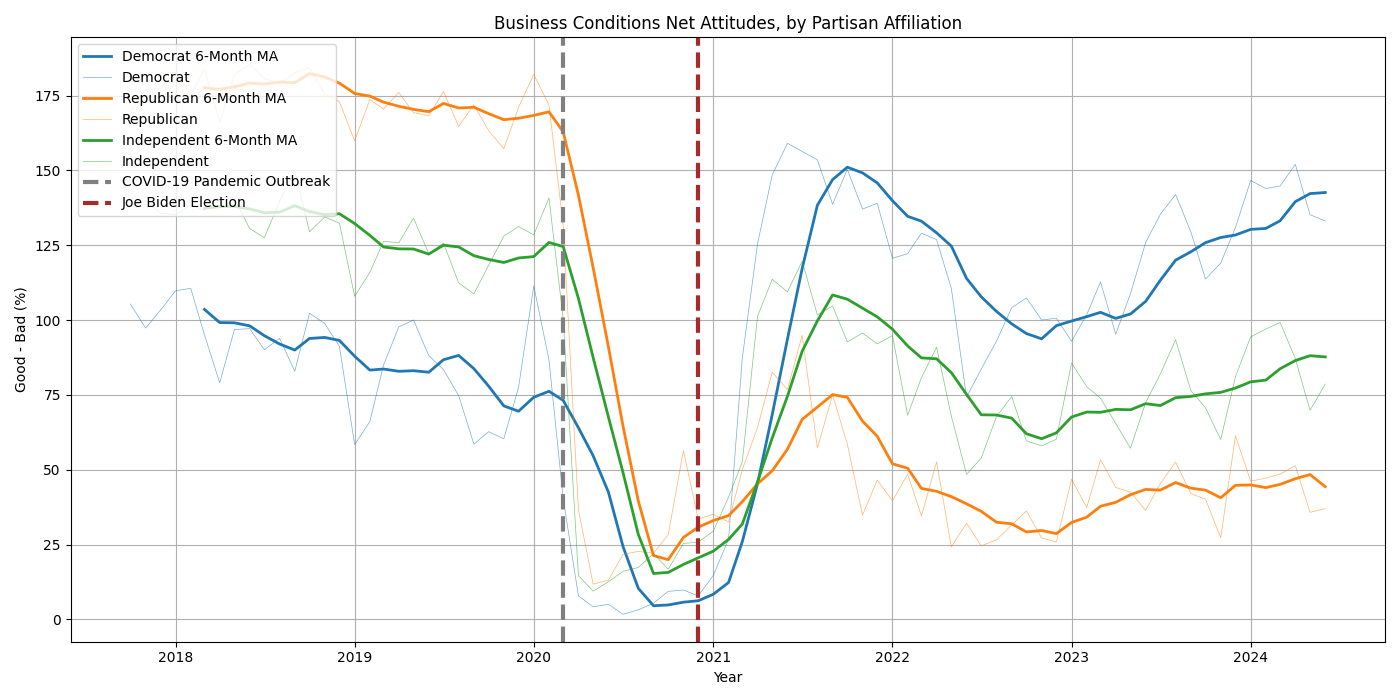
\includegraphics[width=5.5in]{bago_r_time_series.png}\\
\raggedright Unsurprisingly, COVID saw a dramatic drop in broad business conditions, before quickly bouncing back across the board--albeit to different levels. Since about mid-2021, parties' attitudes have seemingly moved in parallel, decreasing until in late-2022 before rebounding. 

\section{Attitudes Towards Home-Buying Conditions}
\centering 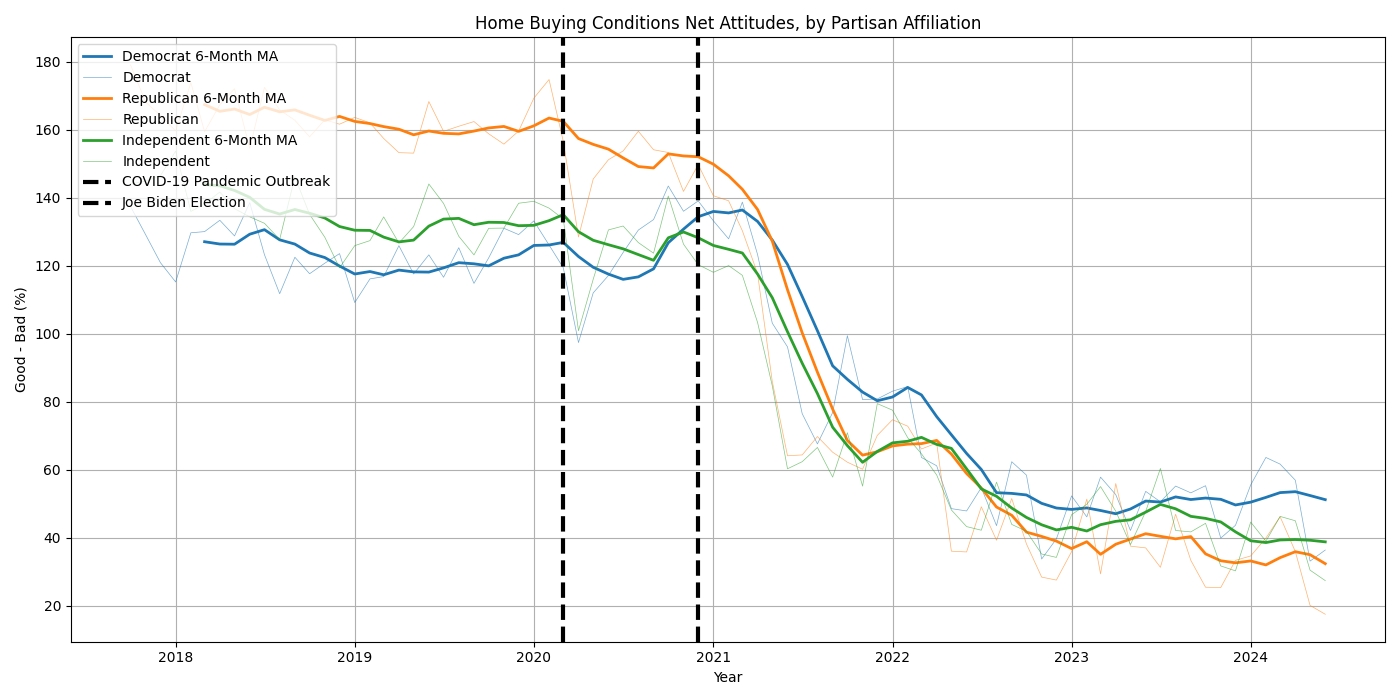
\includegraphics[width=5.5in]{hom_r_time_series.png}\\
\raggedright Attitudes towards home-buying conditions have starkly decreased since Joe Biden's election, irrespective of party. Interestingly, there are two ways we can think of home-buying attitudes: do increasing housing prices motivate respondents to think they can take advantage of ever-increasing real estate prices? Or would respondents expect housing prices to decrease from all-time highs near in the future? 

\subsection{Modeling Voters' Sensitivity to Changes in the Zillow Home Index -- Aggregate Approach}
\centering 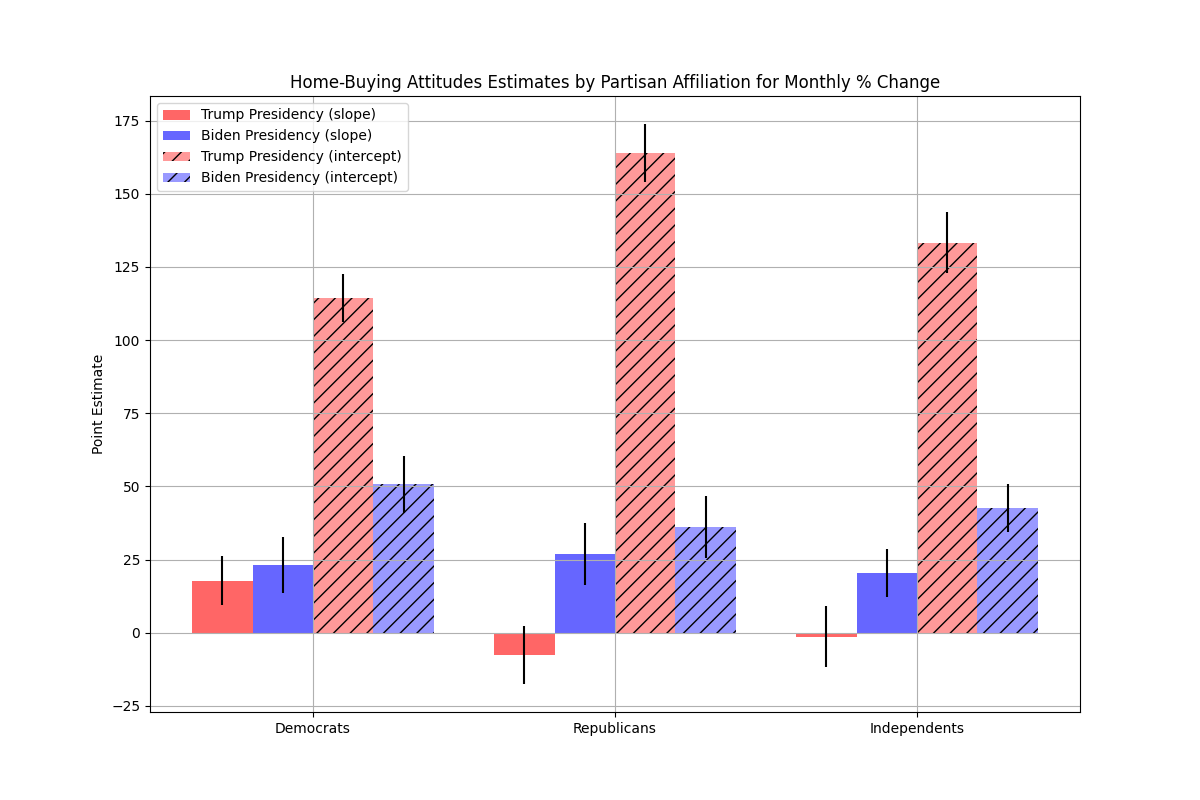
\includegraphics[width=5.5in]{month_hom_party_comp.png} \\
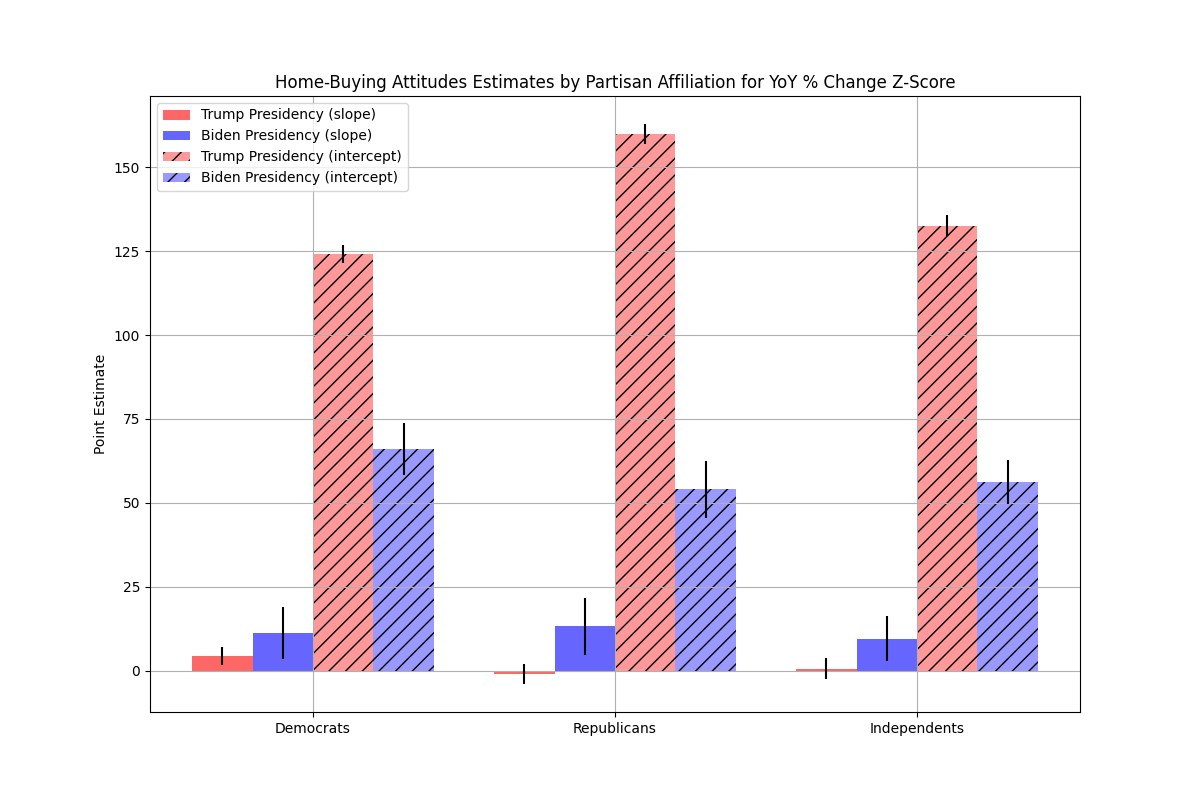
\includegraphics[width=5.5in]{yoy_hom_party_comp.png} \\
\raggedright These results suggest that voters are likelier to think that it is a good time to buy housing the greater the positive change in home values is. 

\subsection{Modeling Voters' Sensitivity to Changes in the Zillow Home Index -- Micro Approach}
\centering 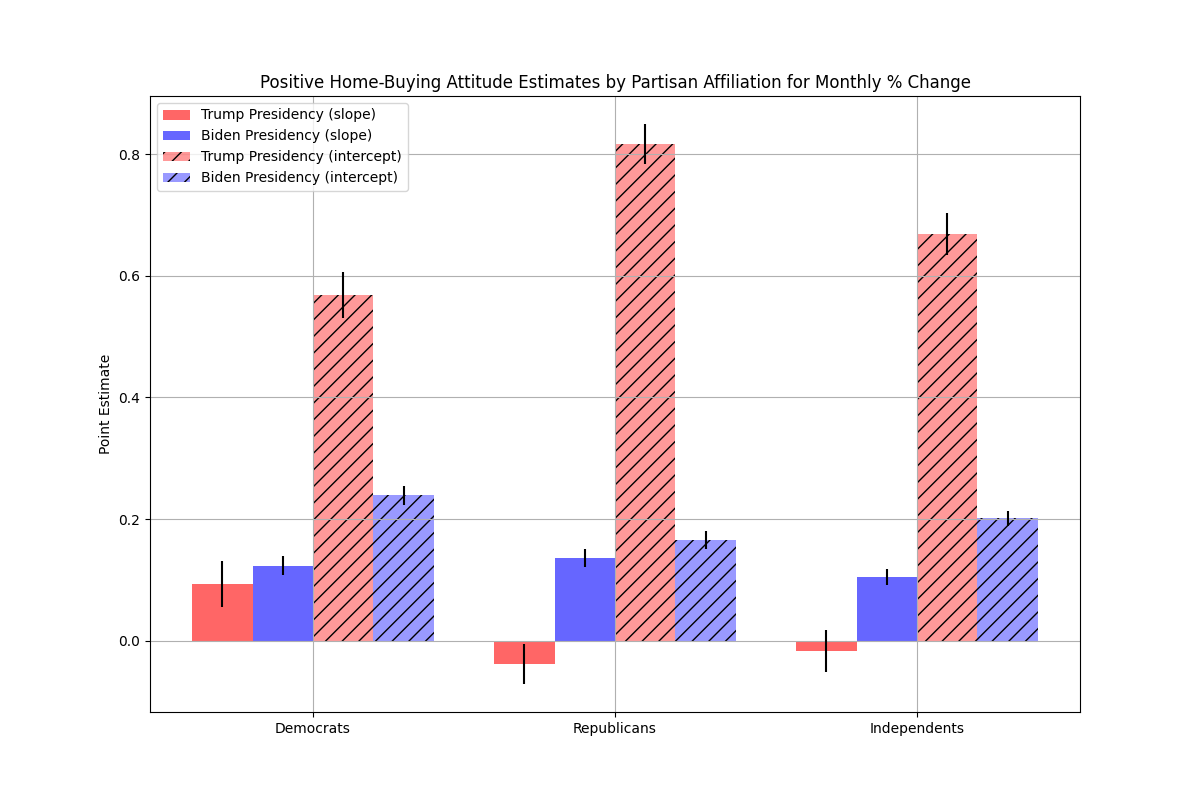
\includegraphics[width=5.5in]{month_hom_party_comp_micro.png} \\
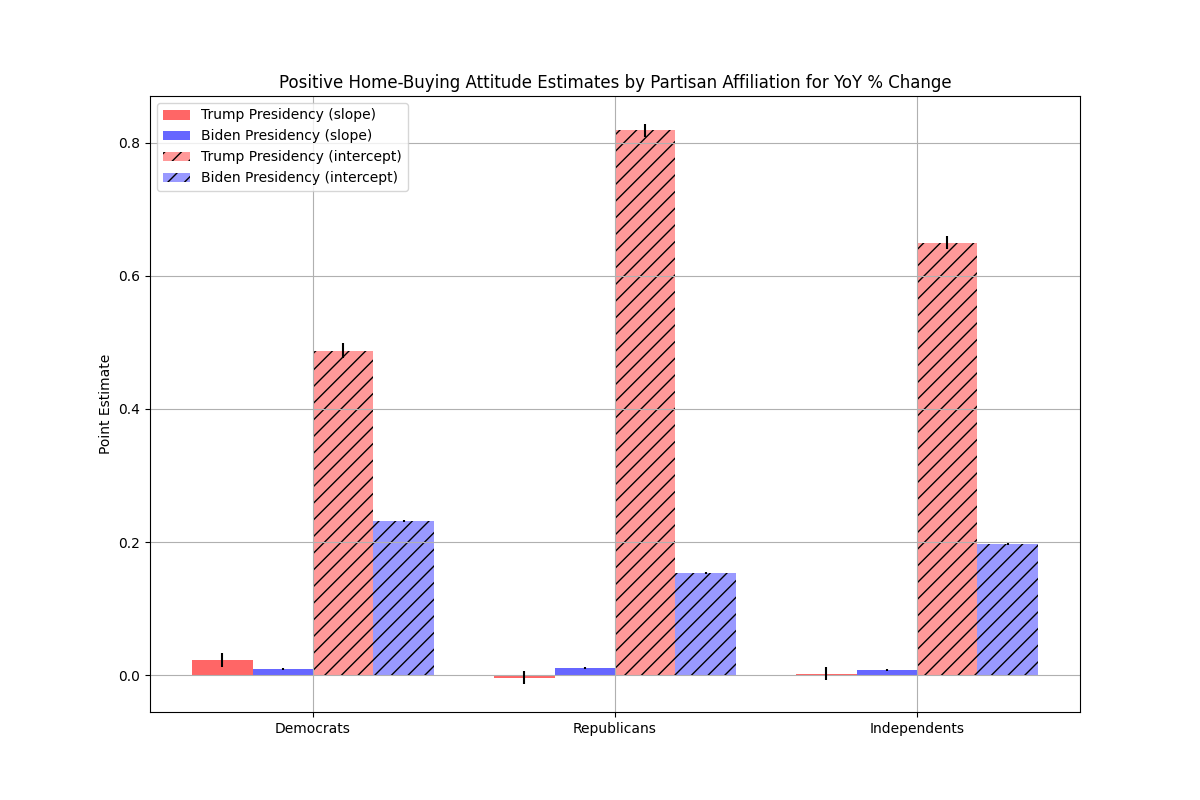
\includegraphics[width=5.5in]{yoy_hom_party_comp_micro.png} \\
\raggedright It appears that voters across the board were likelier to think it was a good time to buy a house during Trump's presidency than Biden's presidency, \textit{regardless} of the actual movement in home value. This would suggest preset biases are motivating home-buying attitudes, rather than observed real-world changes.

\section{Reported Unfavorable News Coverage of Inflation}
\centering 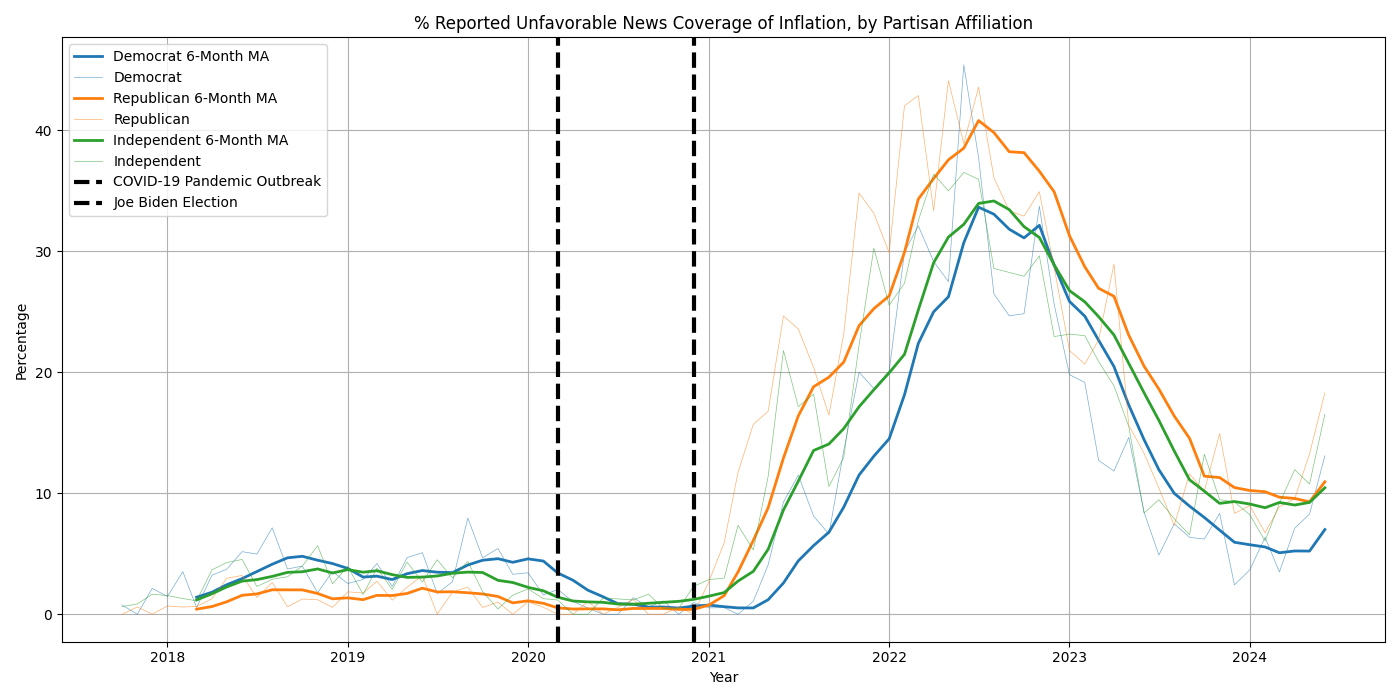
\includegraphics[width=5.5in]{newsrn_u_pri_time_series.png} \\
\raggedright Republicans', Democrats', and Independents' reported unfavorable news coverage of inflation closely follow each other, peaking when observed inflation did in mid-2022 before declining. Democrats appear to have heard less, and later, unfavorable news coverage of inflation.

\subsection{Modeling Voters' Sensitivity to Changes in All-Urban CPI -- Aggregate Approach}
\centering 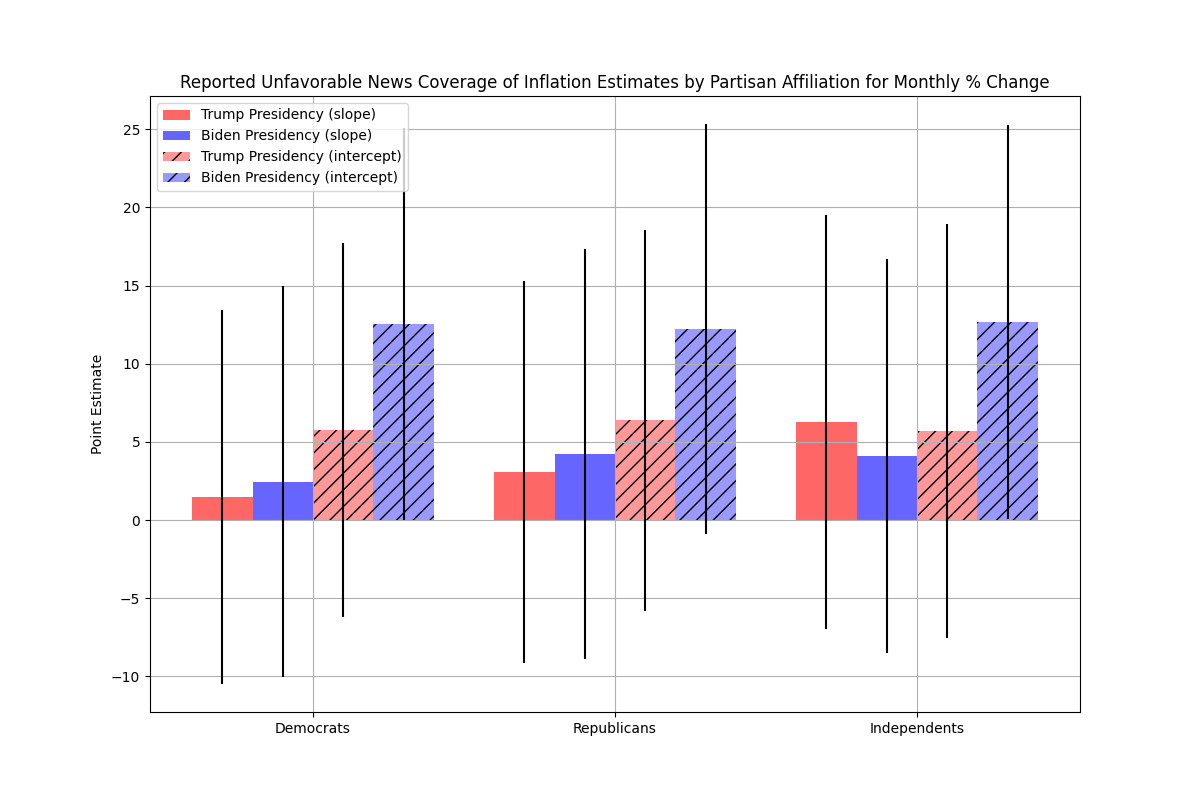
\includegraphics[width=5.5in]{month_news_pri_party_comp.png} \\
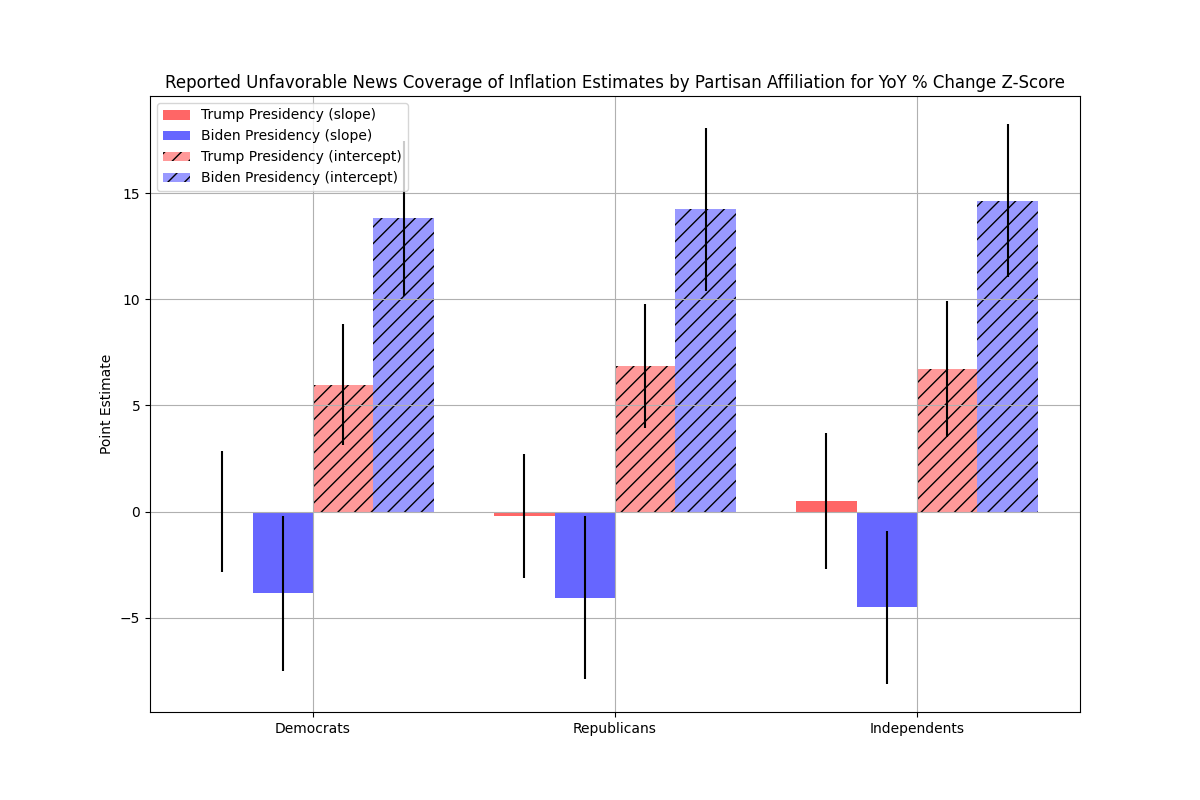
\includegraphics[width=5.5in]{yoy_news_pri_party_comp.png} \\
\raggedright 

\subsection{Modeling Voters' Sensitivity to Changes in All-Urban CPI -- Micro Approach}
\centering 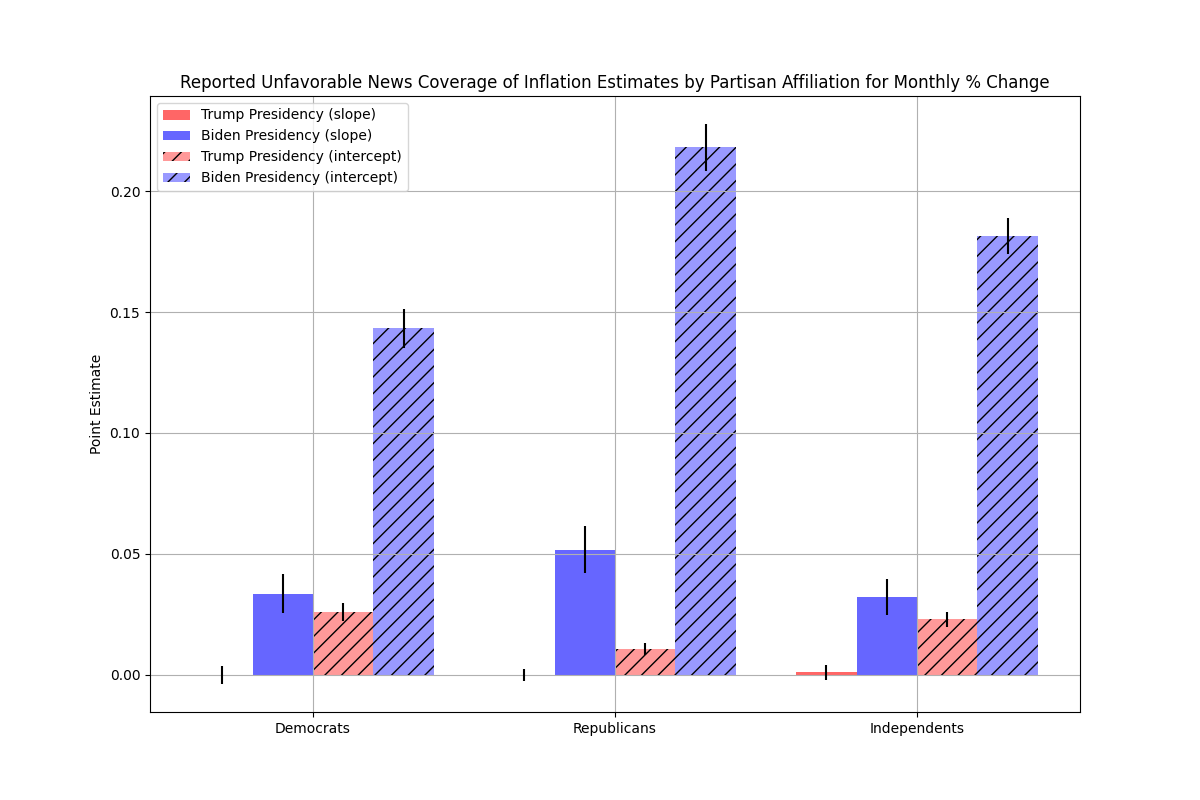
\includegraphics[width=5.5in]{month_news_pri_party_comp_micro.png} \\
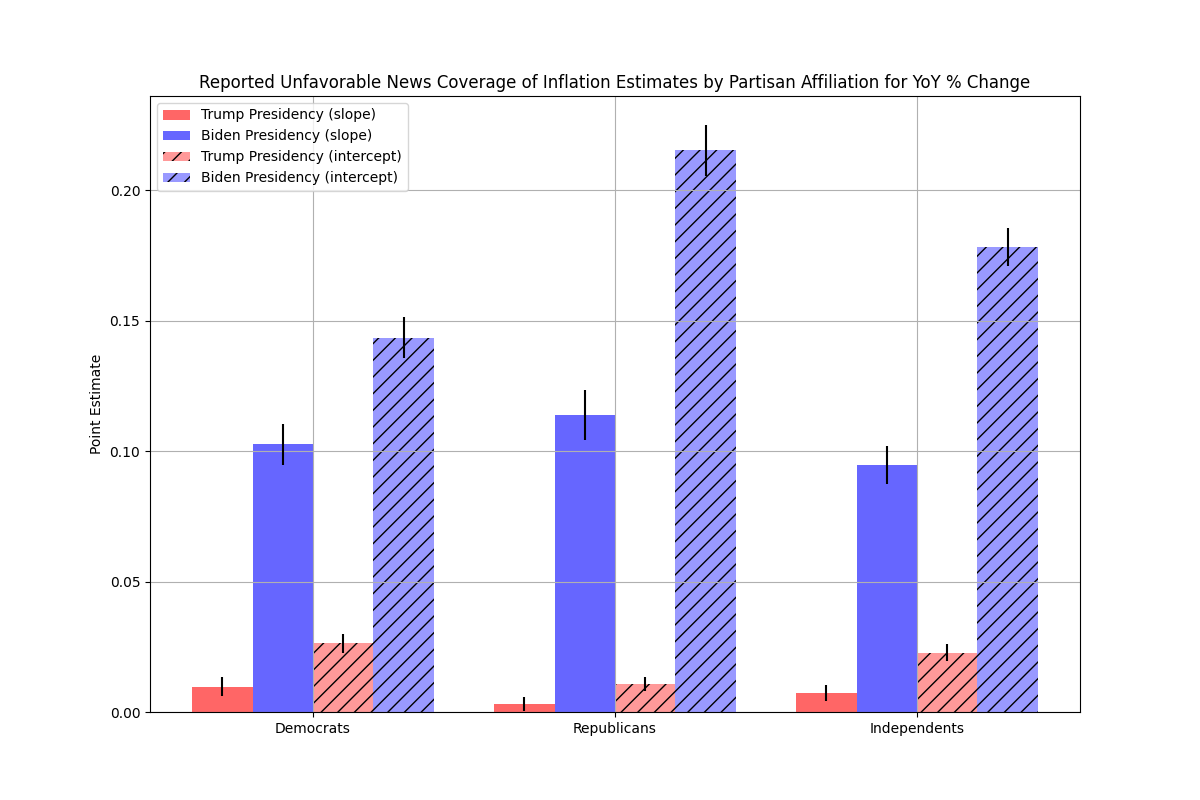
\includegraphics[width=5.5in]{yoy_news_pri_party_comp_micro.png} \\
\raggedright It appears that Republicans were nearly 1.5$\times$ as sensitive to monthly price changes in whether they reported hearing unfavorable news coverage of inflation. They were also 1.5$\times$ as likely to hear this news coverage, even if there was a 0\% monthly increase in prices--suggesting a stark partisan bias in unfavorable news coverage of inflation.

\section{Predicted Likelihood of Positive Returns on Stock Market Index}
\centering 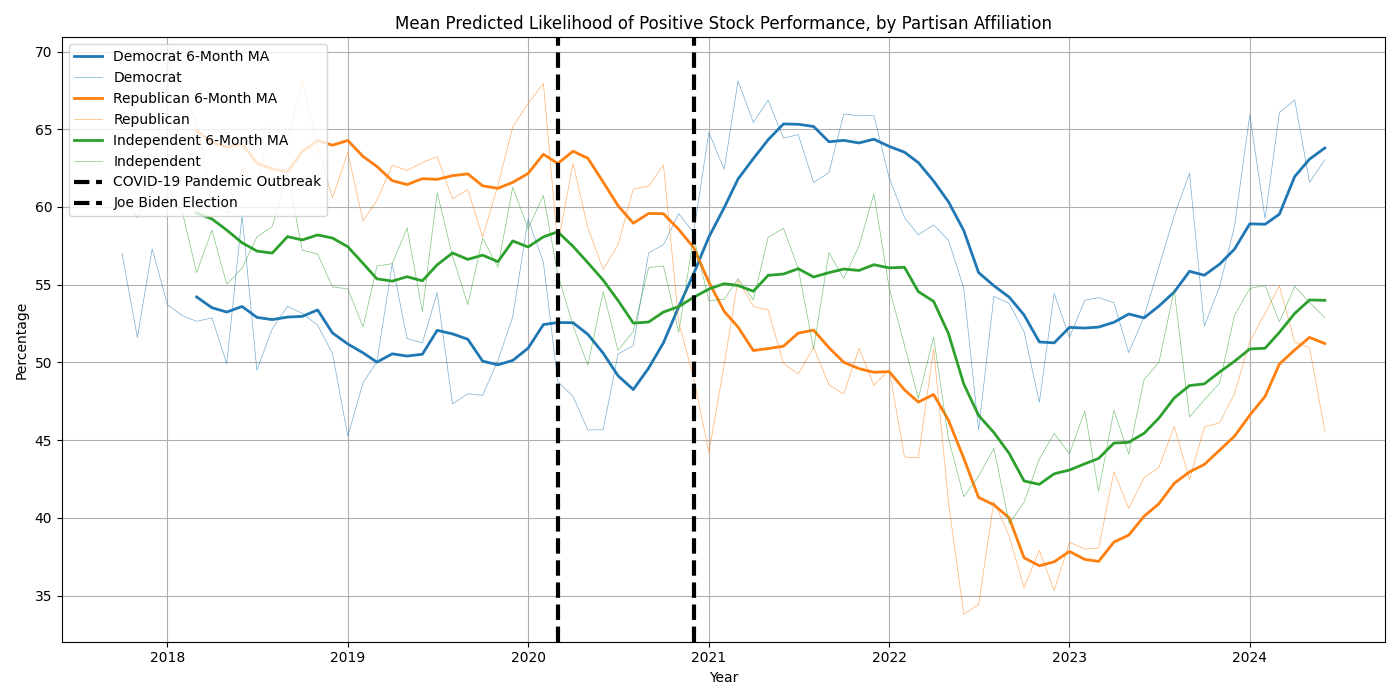
\includegraphics[width=5.5in]{PSTK_time_series.png} \\
\raggedright The pattern in predicted likelihood of positive returns on stock market investment largely mirror the time pattern of general business condition attitudes.

\subsection{Modeling Voters' Sensitivity to Changes in the S\&P 500 Index -- Aggregate Approach}
\centering 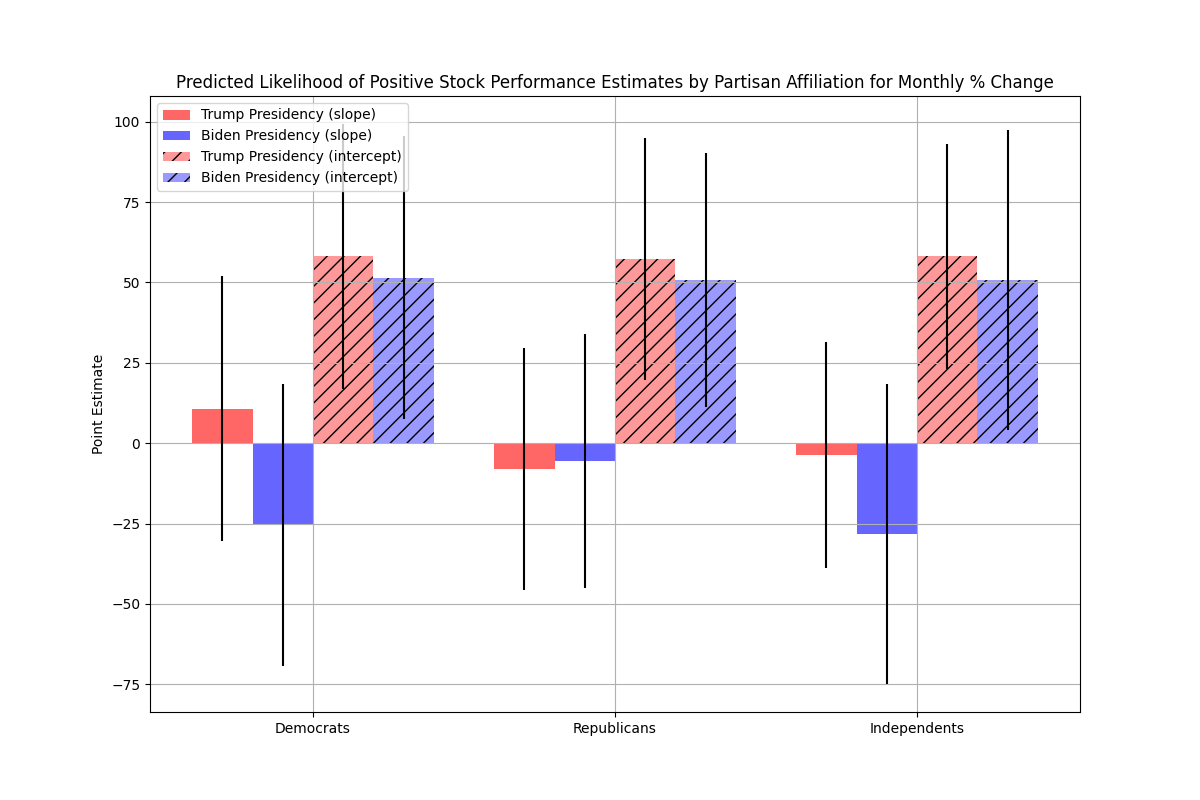
\includegraphics[width=5.5in]{month_pstk_party_comp.png} \\
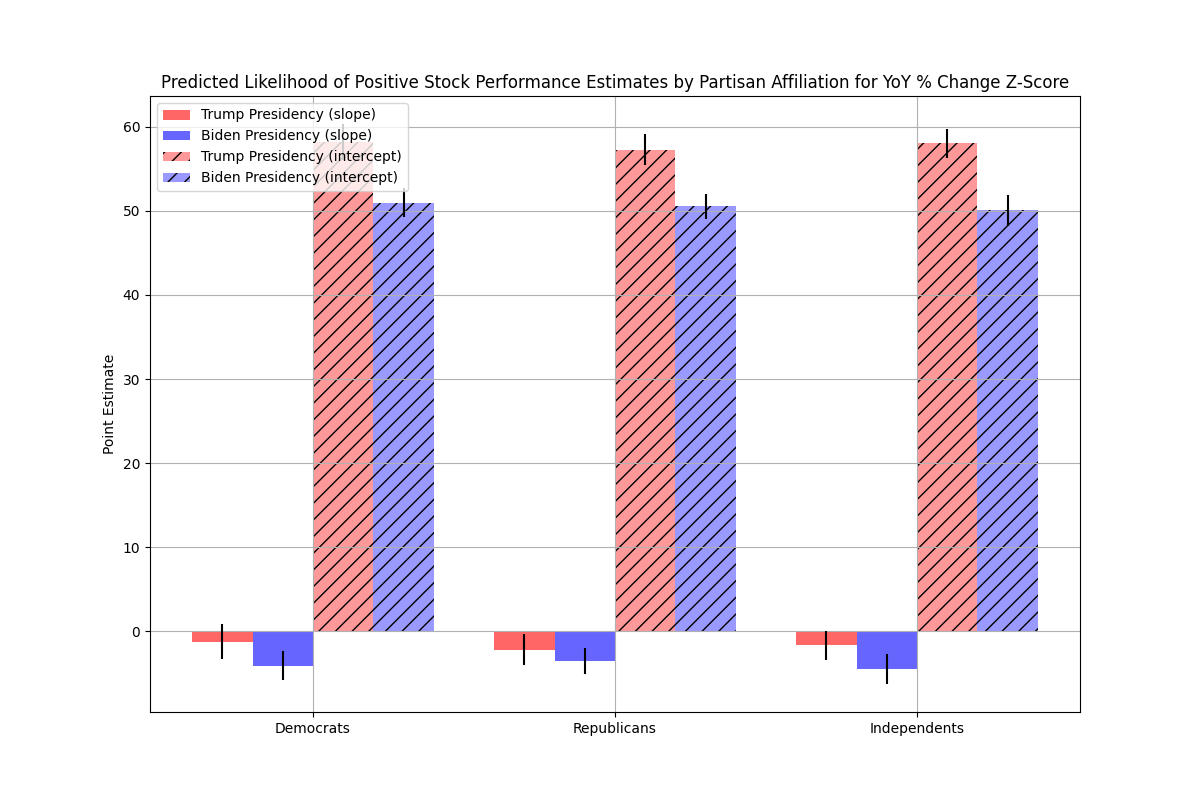
\includegraphics[width=5.5in]{yoy_pstk_party_comp.png} \\
\raggedright ????

\subsection{Modeling Voters' Sensitivity to Changes in the S\&P 500 Index -- Micro Approach}
\centering 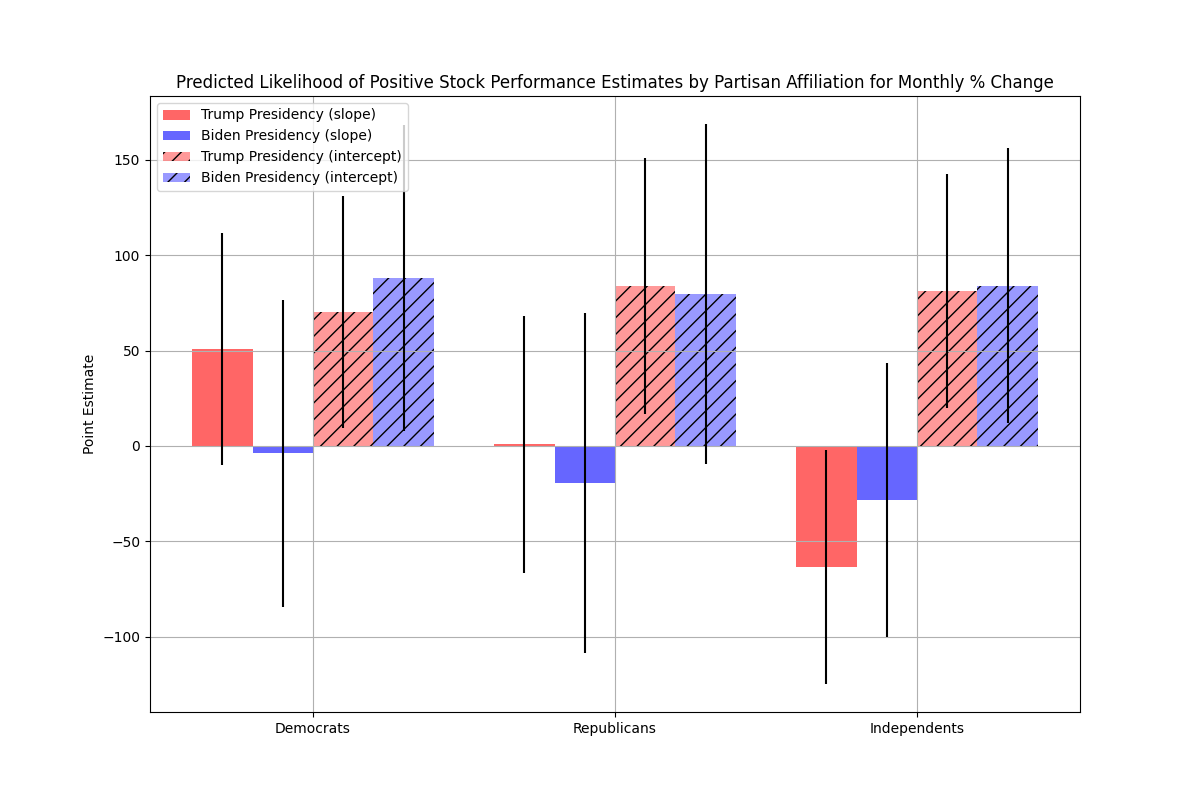
\includegraphics[width=5.5in]{month_pstk_party_comp_micro.png}
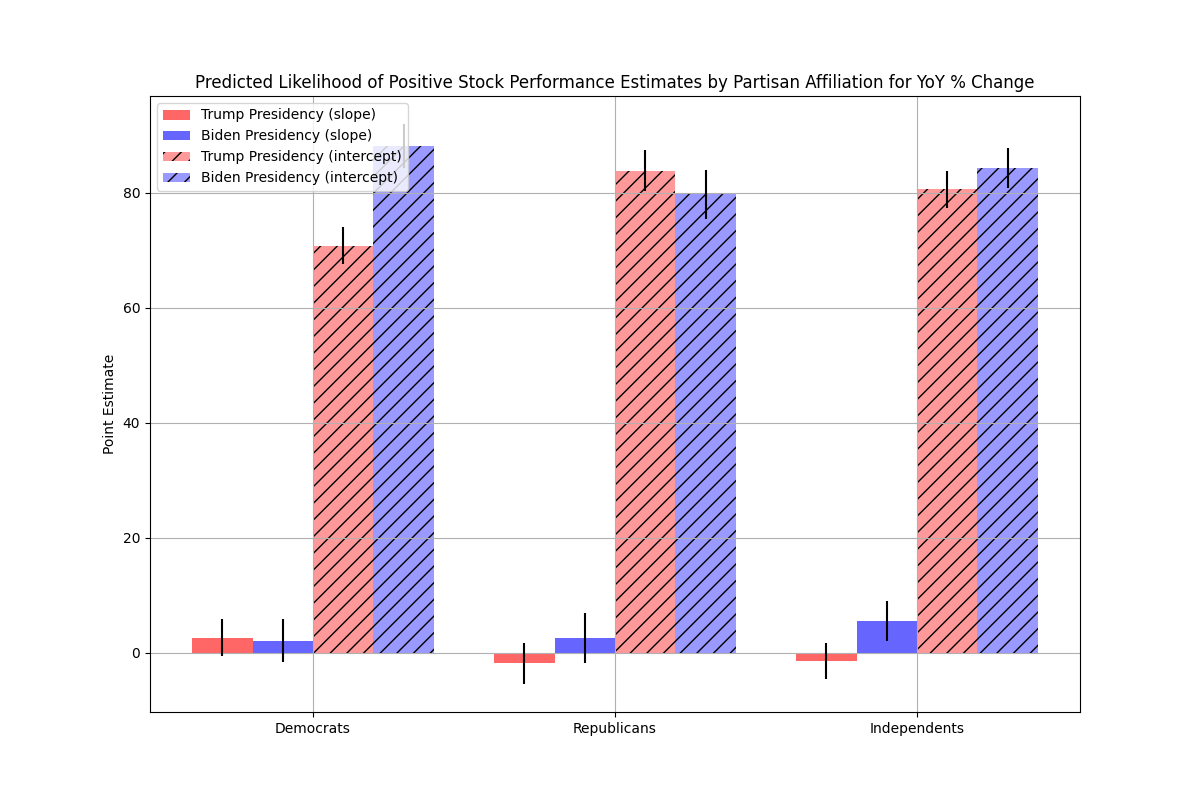
\includegraphics[width=5.5in]{yoy_pstk_party_comp_micro.png} \\
\raggedright 

\section{Attitudes Towards Real Household Income}
\centering 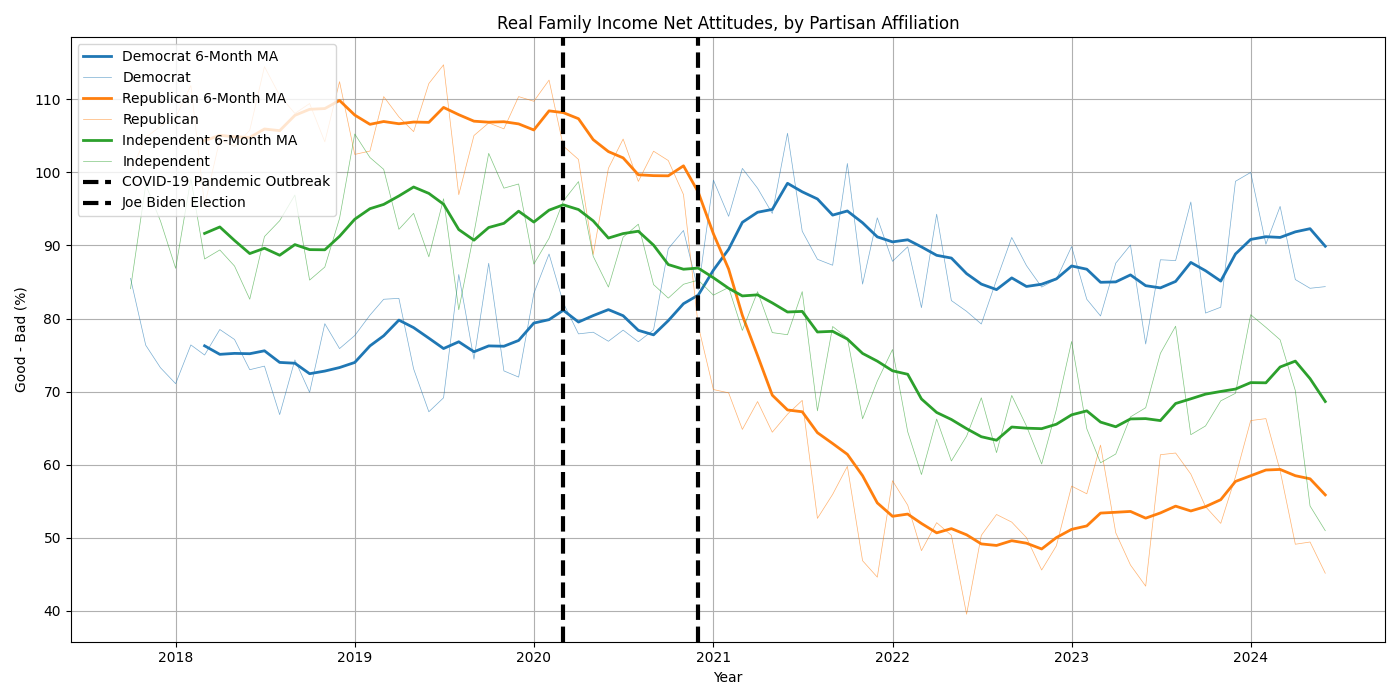
\includegraphics[width=5.5in]{rinc_r_time_series.png} \\
\raggedright This pattern mostly reflects a combination of the trend in reported unfavorable coverage of inflation and general business conditions.

\subsection{Modeling Voters' Sensitivity to Changes in Real Family Income -- Aggregate Approach}
\centering 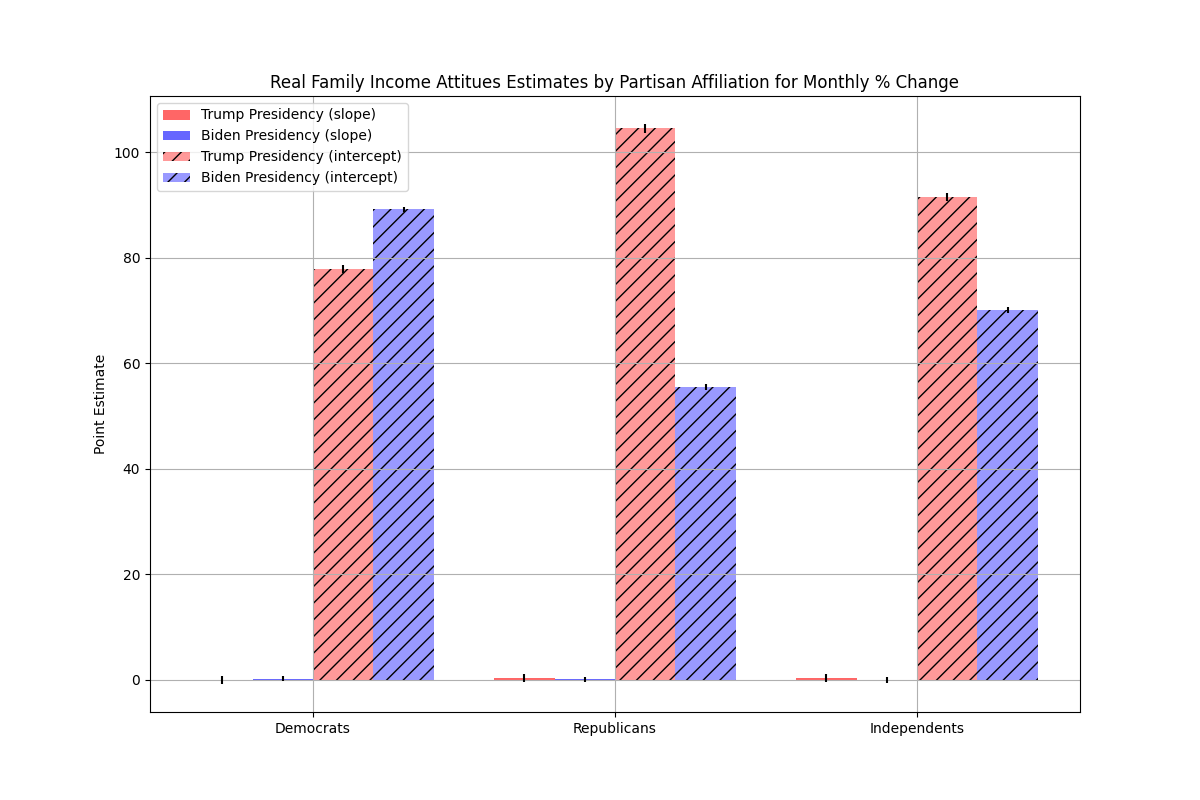
\includegraphics[width=5.5in]{month_rinc_party_comp.png} \\
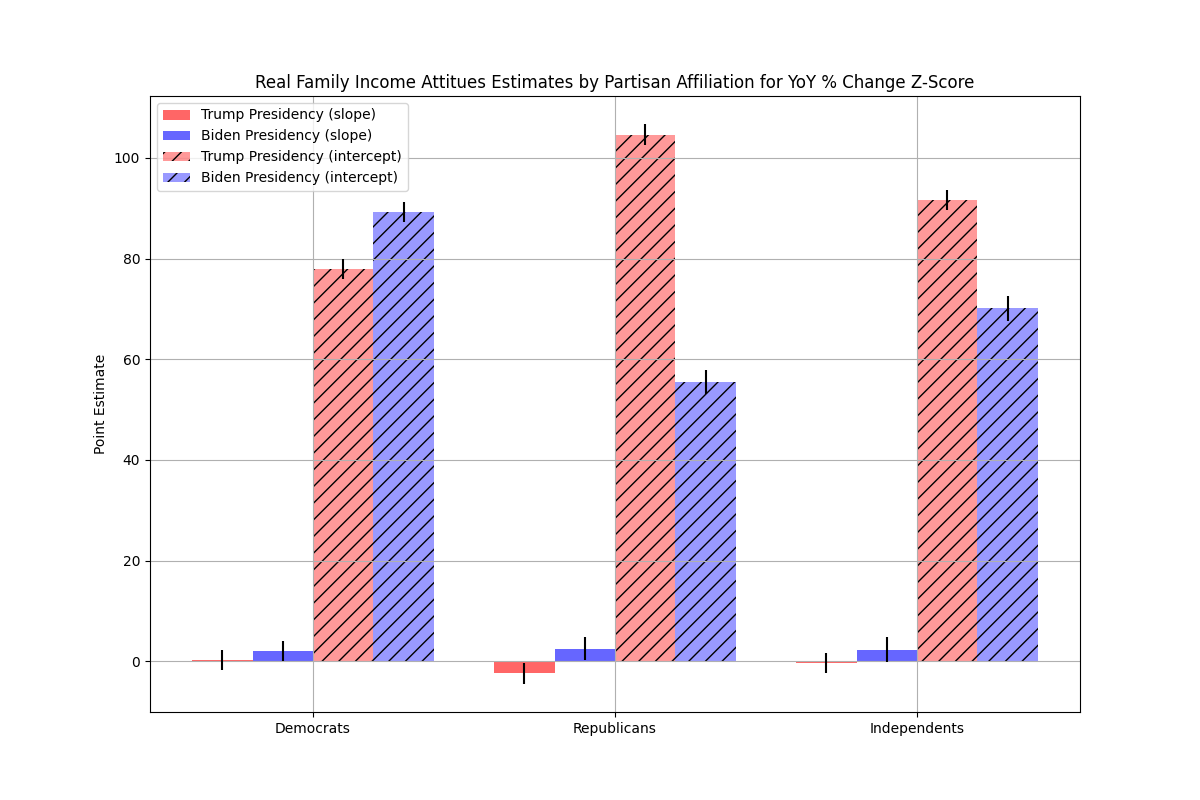
\includegraphics[width=5.5in]{yoy_rinc_party_comp.png} \\
\raggedright This graphic is startling, suggesting that respondents, regardless of party, don't factor observed data \textit{at all} in determining their attitudes towards real family income, even more so than other economic indicators. 

\subsection{Modeling Voters' Sensitivity to Changes in Real Family Income -- Micro Approach}
\centering 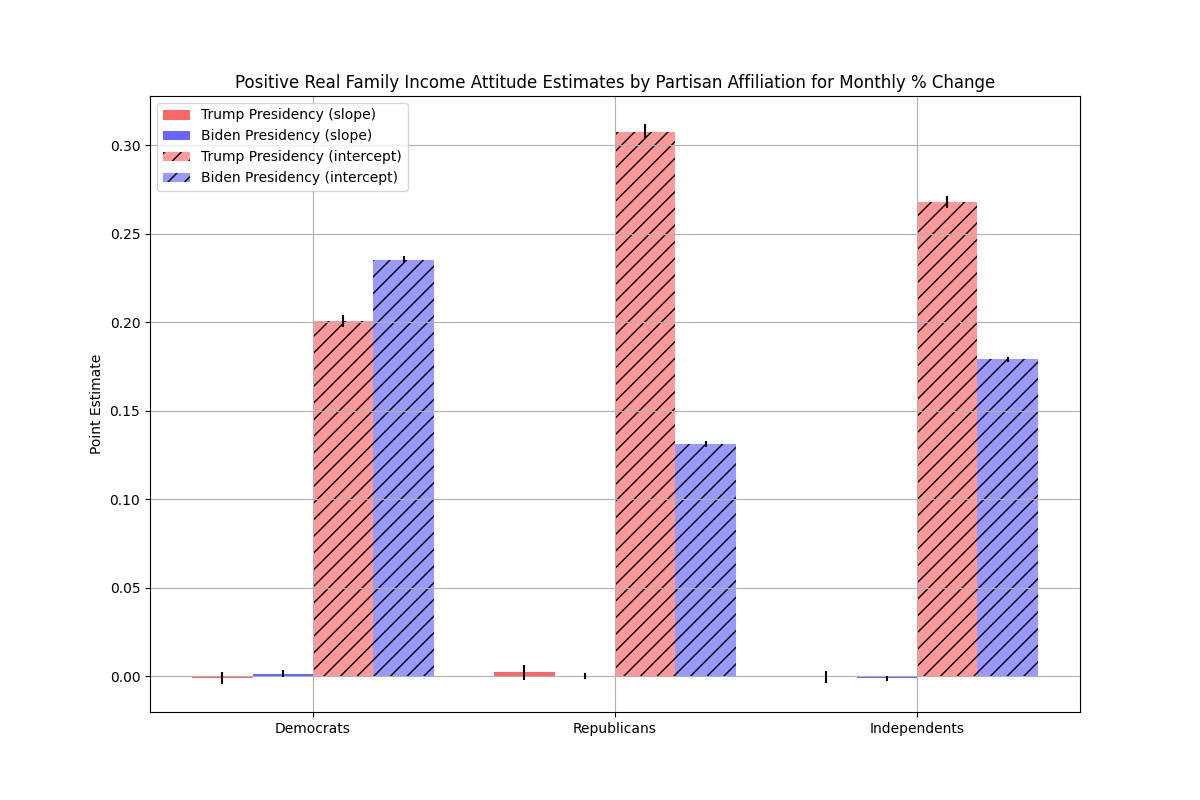
\includegraphics[width=5.5in]{month_rinc_party_comp_micro.png} \\
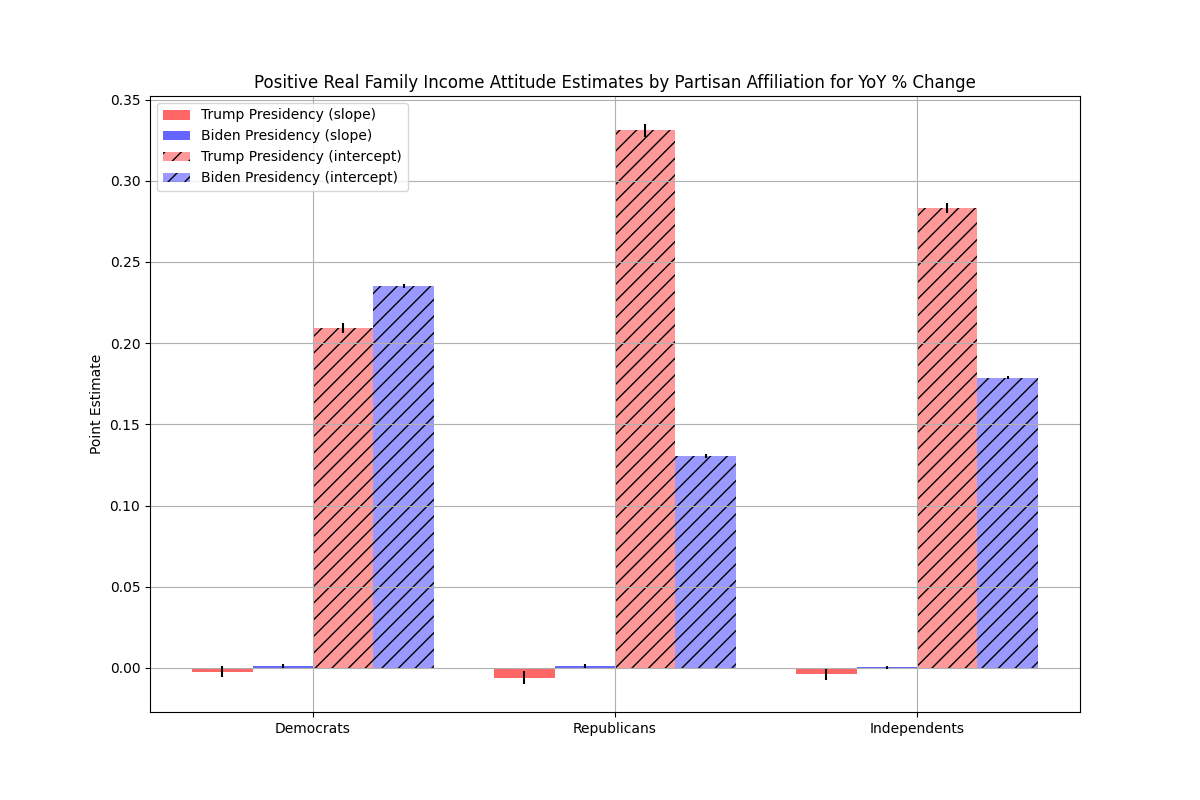
\includegraphics[width=5.5in]{yoy_rinc_party_comp_micro.png} \\
\raggedright Republicans were about 2.5$\times$ likelier to have a positive outlook on real family wages under Trump than President Biden. This political bias is asymmetric; Democrats were only about 1.2$\times$ likelier to have a positive outlook under Biden than Trump.

\section{Attitudes Towards Car-Buying Conditions}
\centering 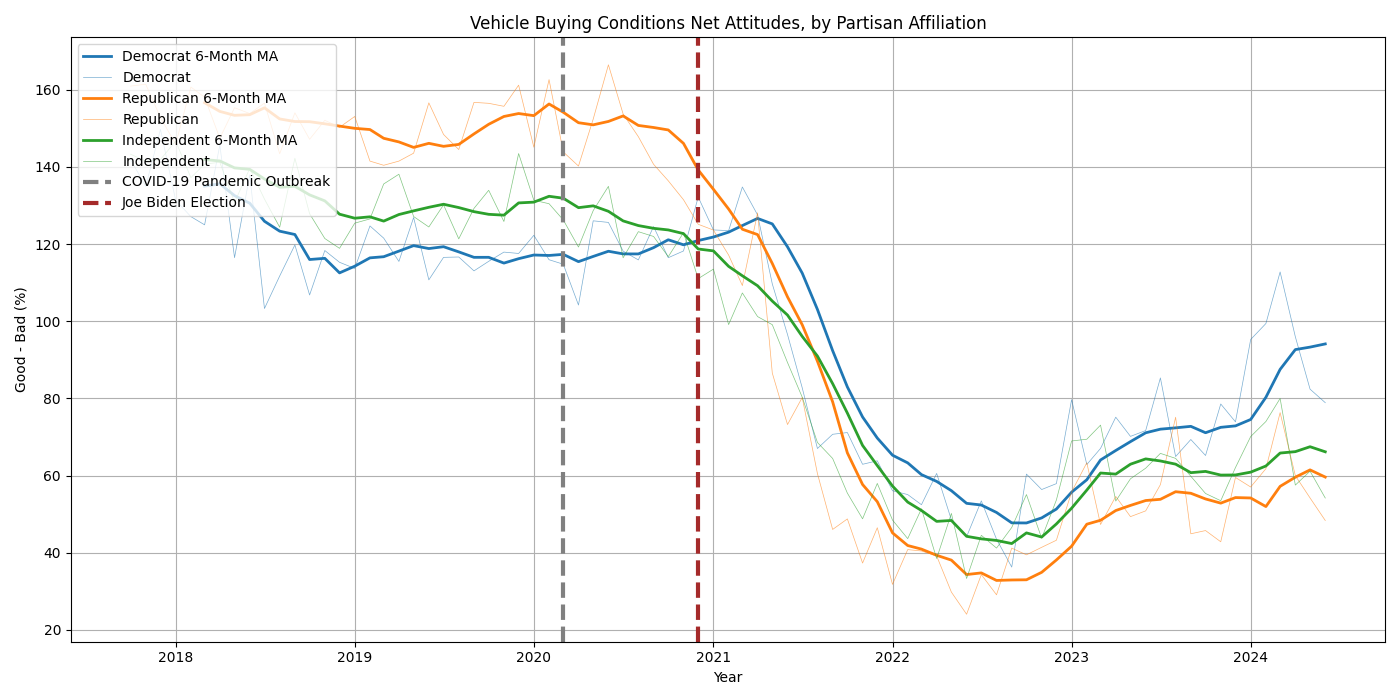
\includegraphics[width=5.5in]{veh_r_time_series.png} \\
\raggedright Interestingly, all respondents, regardless of party, saw their attitudes decline post-Biden's election. However, as interest rate hikes have eased, Democrats' attitudes have recovered much faster than Republicans' or Moderates'. 

\subsection{Modeling Voters' Sensitivity to Changes in Used Car Price Index -- Aggregate Approach}
\centering 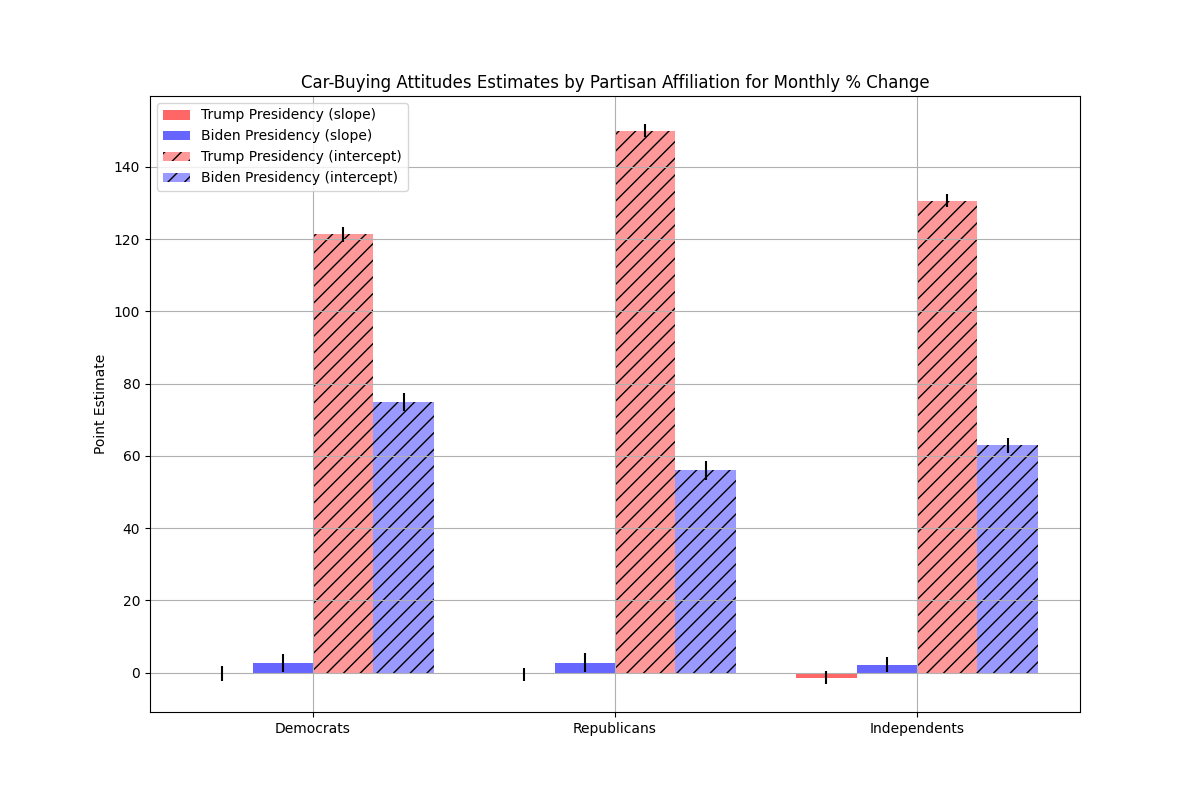
\includegraphics[width=5.5in]{month_car_party_comp.png} \\
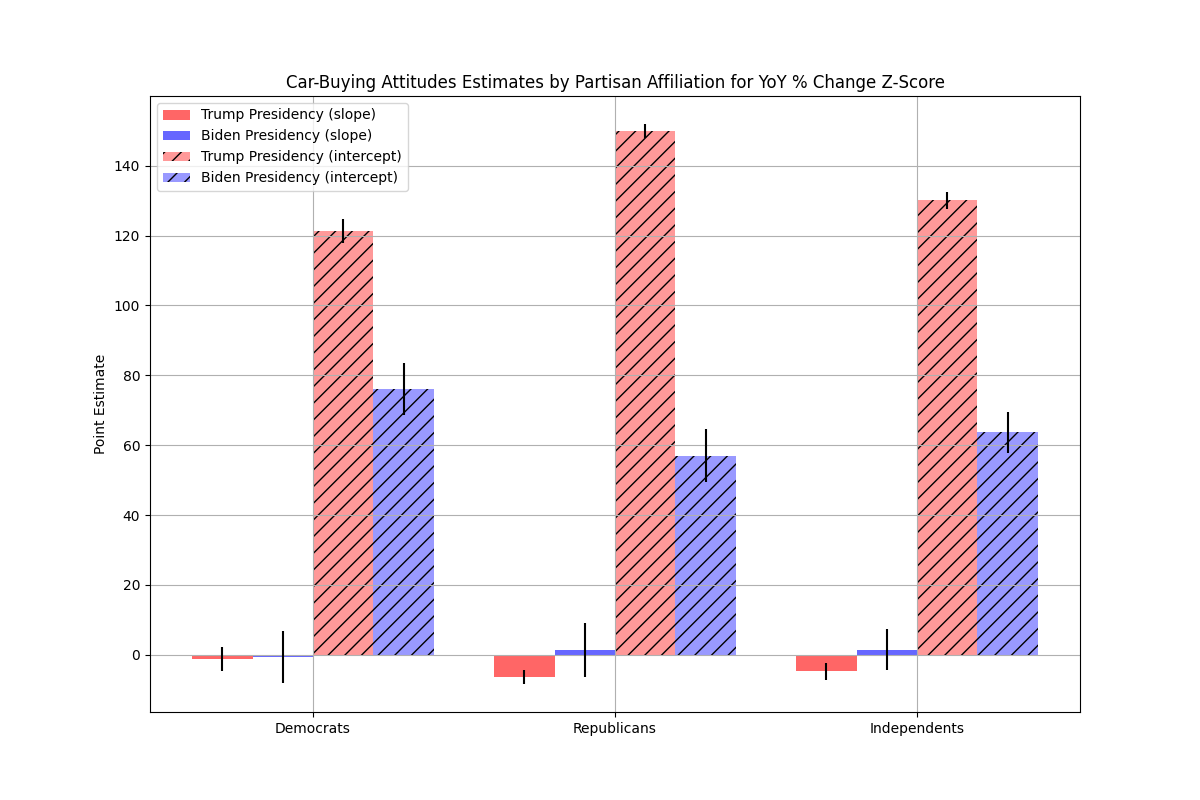
\includegraphics[width=5.5in]{yoy_car_party_comp.png} \\
\raggedright 

\subsection{Modeling Voters' Sensitivity to Changes in Used Car Price Index -- Micro Approach}
\centering 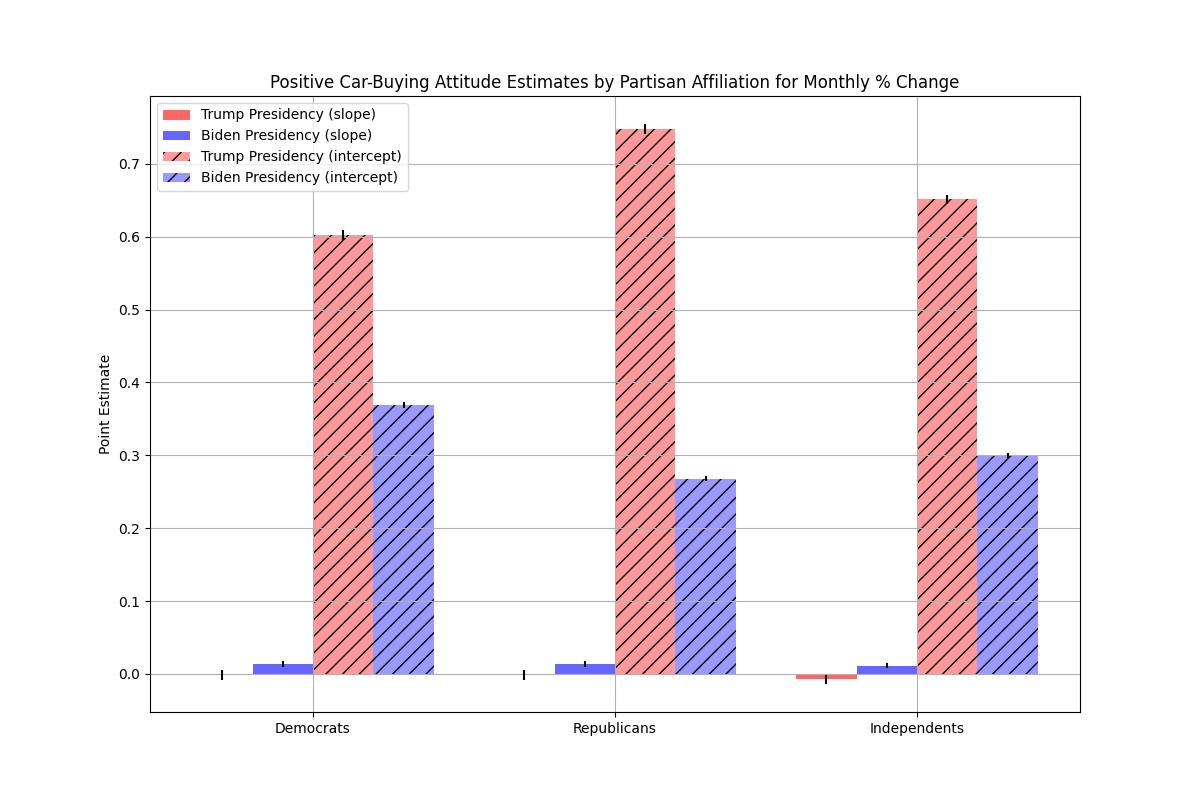
\includegraphics[width=5.5in]{month_car_party_comp_micro.png} \\
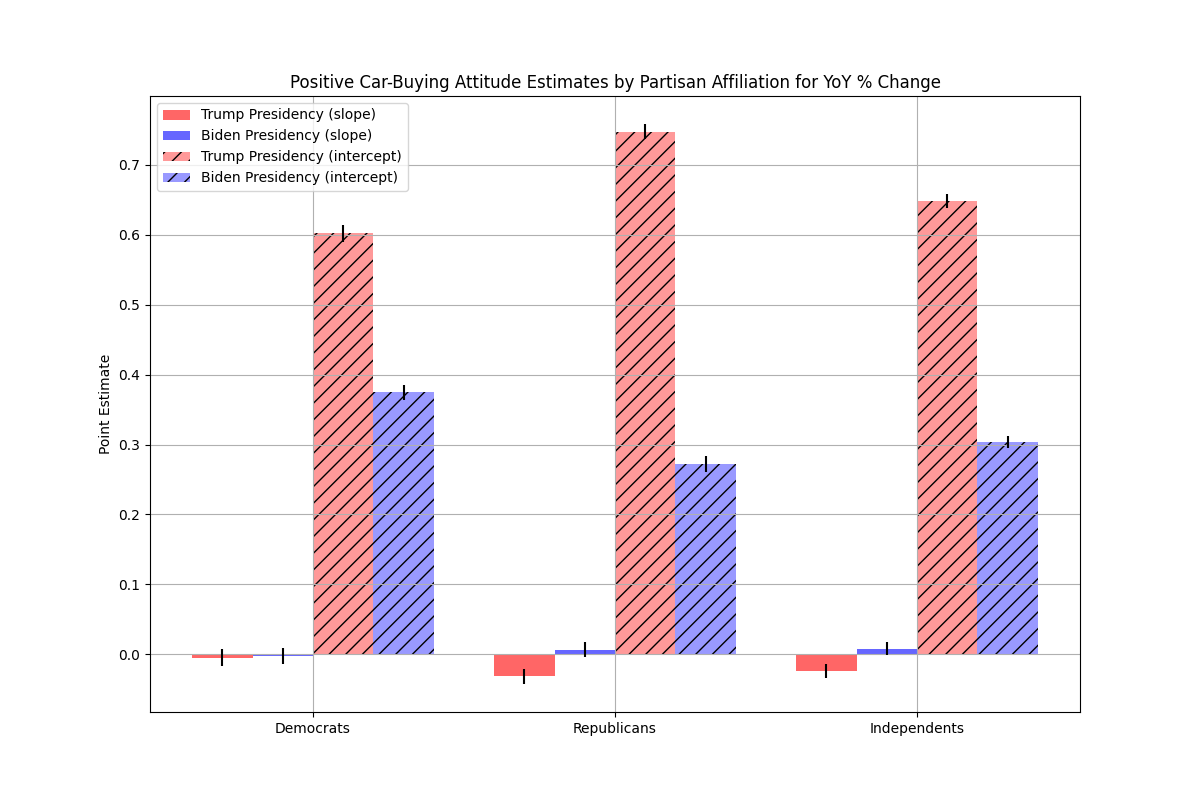
\includegraphics[width=5.5in]{yoy_car_party_comp_micro.png} \\
\raggedright Much like real family income, the slope terms in these models are near-zero and very insignificant. For car-buying attitudes, however, respondents' pre-set biases move in the same direction, regardless of party--although the magnitudes vary. Even if car prices see a 0\% change, Republicans were approximately $2.5\times$ likelier to think it was a good time to buy a car under Trump than under Biden. For Democrats, they were approximately $1.7\times$ likelier to think it was a good time to buy a car under Trump than under Biden.

\end{document}